\paragraph{La dimension rappel}
\lecture{13}{2024-10-29}{Base, noyau, image}{}

\begin{definition}
    Un espace vectoriel $V$ est de dimension nulle si et seulement si $V = \{0\}$.
\end{definition}
0 est un vecteur linéairement dépendant, il ne peut donc faire partie d'aucune base. La convention dite auparavant est : $Vect\{\emptyset\} = \{0\}$. Ainsi l'ensemble vide est une famille libre de générateur de $\{0\}$.

\begin{theoreme}[de la base incomplète]
    Soit $V$ un espace vectoriel de dimension $n$ et $\{e_1, \dots, e_k\}$ une famille libre de vecteurs de $V$. Il existe alors des vecteurs $e_{k+1}, \dots, e_n$ tels que ($e_1, \dots, e_n)$ forme un base de $V$.
\end{theoreme}
\begin{framedremark}
    Attention à ne pas confondre une base et des vecteurs c'est pour ça qu'ici on choisit des parenthèse pour une base et des ac?dallades pour une famille de vecteurs.
\end{framedremark}

\subparagraph{preuve} Si $(e_1, \dots, e_k)$ forme déjà une base de $V$, on s'arrête là.\\
Sinon il existe un vecteur $e_{k+1}$ qui n'est pas dans $Vect\{e_1, \dots, e_k\}$. J'affirme que $\{e_1, \dots, e_k, e_{k+1}\}$ est libre.
\\
\begin{itemize}
    \item En effet si $\alpha_1e_1, \cdots + \alpha_ke_k + \alpha_{k+1}e_{k+1} = 0$ alors $\alpha_{k+1} = 0$ car $e_{k+1}$ n'est pas combinaison linéaire des autres $e_j$ par construction.
    \item Ainsi $\alpha_1e_1 + \cdots + \alpha_ke_k  = 0$.
    \item Comme la famille de départ est libre, tous les $\alpha_i$ sont nuls
    \item On peut donc ajouter $e_{k+1}$ à la famille $\{e_1, \dots, e_k\}$
\end{itemize}
On continue ce processus inductif jusqu'à compter $n$ vecteurs


\begin{exemple}
Dans $M_{2 \times 3}(\mathbb{R})$, $dim = 6$ on prend les quatre matrices:
\[A = \begin{pmatrix}
    1 & 0 & 0 \\ 1 & 1 & 0
\end{pmatrix} ,  B = \begin{pmatrix}
    1 & 1 & 0 \\ 0 & 1 & 0
\end{pmatrix}, C  = \begin{pmatrix}
    1 & 0 & 0 \\ 0 & 1 & 0
\end{pmatrix}, D = \begin{pmatrix}
    1 & 0 & 0 \\ 0 & -1 & 0
\end{pmatrix}\]
Si on écrit ces matrices dans la base canonique de $M_{2\times 3}(\mathbb{R}), \mathcal{C}an$ et qu'on créer une matrice avec les lignes de ces vecteurs on a:
\[M = \begin{pmatrix}
    1 & 0 & 0 & 1 & 2 & 0\\
    1 & 1 & 0 & 0 & 1 & 0\\
    1 & 0 & 0 & 0 & 1 & 0 \\
    1 & 0 & 0 & 0 & - 1 & 0 \\
\end{pmatrix} \to \begin{pmatrix}
    1 & 0 & 0 & 0 & 1 & 0\\
    0 & 1 & 0 & 0 & 0 & 0\\
    0 & 0 & 0 & 1 & 0 & 0 \\
    0 & 0 & 0 & 0 & - 2 & 0 \\
\end{pmatrix} \]
On voit ici qu'il y a deux vecteurs ne sont pas des colonnes pivots ($e_{13}, e_{23})$, il ne sont donc pas combinaison linéaire de $A'$ ni de $A$.
\\
Et donc $(A, B, C, D, e_{13}, e_{23})$ est une base de $M_{2\times 3}(\mathbb{R})$.
\begin{framedremark}
    On a rajouter $e_{13}$ et $e_{23}$ car il ne sont pas combinaison linéaire.
\end{framedremark}
\end{exemple}

\paragraph{Deux points de vue sur les bases}
Soit $V$ un espace vectoriel de dimension $n$. Une \textcolor{red}{base} est une famille ordonnée de générateurs libre de $V$. Nous avons vu que toute base est composée du même nombre $n$ de vecteurs.
\\
\textbf{Critères}
\begin{itemize}
    \item Une famille libre $\mathcal{L}$ de $n$ vecteurs forme une base de $V$
    \item une famille génératrice $\mathcal{G}$ de $n$ vecteurs forme une base de $V$.
\end{itemize}
\\
Soit $\mathcal{F}  = \{f_1, \dots, f_k\}$ une famille génératrice de $V$ et $\mathcal{B} = (e_1, \dots, e_n)$ une base de $V$. Pour extraire une base de $\mathcal{F}:$
\begin{itemize}
    \item trouver les composantes des $f_j$ dans la base $\mathcal{B}$
    \item Ecrire la matrice $F$ dont les \textcolor{red}{colonnes} sont les $(f_j)_{\mathcal{B}}$.
    \item Echelonner $F$. (sur les lignes)
    \item Ne garder que les $n$ colonnes pivots de $F$.
    
\end{itemize}

\begin{exemple}
    Extraire de la famille $\{1 - t, -1 + t^2, t^2 - t, 1 + t, t^2 + 1\}$ une base de $\mathbb{P}^2$. On choisit la base canonique de $\mathbb{P}^2$:
    \[(1-t)_{\mathcal{C}an} = \begin{pmatrix}
        1 \\ -1 \\ 0
    \end{pmatrix}, (-1+t^2)_{\mathcal{C}an} = \begin{pmatrix}
        -1 \\ 0 \\ 1
    \end{pmatrix}, \dots \text{et on écrit:}\]
    \[A = \begin{pmatrix}
         1 &-1&0 & 1 & 1 \\
        -1&0&-1&1&0\\
         0&1&1&0&1
    \end{pmatrix} \to \begin{pmatrix}
         1 &-1&0 & 1 & 1 \\
        0&-1&-1&2&1\\
         0&0&0&2&2
    \end{pmatrix}\]
    La prochaine étape après avoir échelonner et de ne garder que les $n$ colonnes pivots de $F$, on voit donc choisir ici $3$ vecteurs qui ont chacun un pivot sur une ligne différente, les colonnes $1, 2, 4$. Ce qui donne:
    \[\mathcal{B} = (1-t, 1+t^2, 1+t)\] \textcolor{red}{Attention!}, on prend les colonnes qui sont les vecteurs et non directement les valeurs trouvées lorsqu'on échelonne. on prend les vecteurs qui se trouvaient sur les colonnes $1, 2, 4$.
\end{exemple}

\paragraph{Comment compléter une base}
Soit $\mathcal{F} = \{f_1, \dots, f_k\}$une famille libre de $V$ dont on a une base $(e_1, \dots, e_n)$. Pour compléter $\mathcal{F}$ en une base:
\begin{itemize}
    \item Trouver les composantes des $f_j$ dans la base $\mathcal{B}$.
    \item Ecrire la matrice $F$ dont les \textcolor{red}{lignes} sont les $(f_j)_{\mathcal{B}}$
    \item Echelonner $F$. (comme d'habitude)
    \item Ajouter les vecteurs $e_i$ pour les valeurs de $i$ qui ne son pas des colonnes pivot.
\end{itemize}

\begin{exemple}
    Compléter la famille $\{\vec{e_2} -\vec{e_1}, \vec{e_3} -\vec{e_1}, \vec{e_4} - \vec{e_1}\}$ en un base de \R$^4$.
    \[A = \begin{pmatrix}
        -1 & 1 & 0 & 0 \\
        -1&0&1 & 0\\
        -1&0&0 & 1
    \end{pmatrix}\to \begin{pmatrix}
        -1 & 0 & 0 & 1 \\
        0&1&0 & -1\\
        0&0&1 & -1
    \end{pmatrix} \]
    On voit qu'il y a pas de pivot sur la dernière colonne.
\end{exemple}


\paragraph{Rappels application linéaires:}
Soit $V$ et $W$ deux espaces vectoriels.
\begin{definition}[application linéaire]
    Une application $T : V \to W$ est \textcolor{red}{linéaire} si
    \begin{enumerate}
        \item $T(u + v) = Tu + Tv$ pour tous $u, v \in V$
        \item $T(\alpha v) = \alpha Tv$ pour tous $v \in V$ et $\alpha \in $\R
    \end{enumerate}
\end{definition}
\begin{exemple}
    \begin{enumerate}
        \item La dérivée $D : \mathcal{C}^\infty(\mathbb{R}) \to \mathcal{C}^\infty(\mathbb{R}) $ des applications $\infty-$dérivables est linéaire. Ici $D(f) = f'$.
        \\
        En effet $(f+g)' = f' + g'$ et $(\alpha\cdot f)' = \alpha f'$
        \item La dérivée $D : \mathbb{P}_n \to \mathbb{P}_{n-1}$ est linéaire. Ici $D(p) = p'$. En particulier $D(t^k) = kt^{k-1}$
        \\
        On peut prendre cela comme définition et "\textit{étendre par linéarité}", c'est à dire définir
        \[D(a_nt^n + a_{n-1}t^{n-1} + \cdots + a_1t + a_0) \text{ comme }\]
        \begin{formule}
            \[n\cdot a_n t^{n-1} + (n-1)\cdot a_{n-1}t^{n-2} + \cdots + a_1 \]
        \end{formule}
    \end{enumerate}
    \begin{framedremark}
        On voit ici que l'application $D(1) = 0$ ce qui signifie plusieurs choses qui sont équivalentes. On voit en premier lieu que l'application n'est pas injective et aussi que le noyau n'est clairement pas nul et qu'il est même de dimension $1$ qui est le vecteur des constantes.
    \end{framedremark}

    Contre exemple:
    \\ 
    L'application $C : \mathbb{P}_2 \to \mathbb{P}_4$ définie par 
    \begin{formule}
    \[p \to p^2\]
    \end{formule}
    n'est pas linéaire. En effet on voit par exemple que:
    \[C(2t) = (2t)^2 = 4t^2 \neq 2t^2 = 2C(t)\]
    \begin{framedremark}
        Généralement, les applications linéaires n'aiment pas quand on les met au carrées.
    \end{framedremark}
\end{exemple}


\paragraph{Noyau}
Soit $T: V \to W$ une application linéaire.
\begin{definition}
    Le \textcolor{red}{noyau} de $T$ est le sous-ensemble $Ker T = \{v \in V | Tv = 0\}$.
\end{definition}
Ce qui veut dire que le noyau est le sous-ensemble des vecteurs qui ont pour image le zéro. donc si on prend par exemple les dérivées, on voit que tout les constantes ont la même image qui est 0 donc le noyaux de l'application linéaire des dérivées et le vecteur des constantes.
\begin{exemple}
    Soit $T: \mathbb{R}^2 \to \mathbb{R}^2$ la projection orthogonale sur l'axe $x = y$.
    On voit que c'est la droite $x$ on a donc que:
    \[T(\vec{e_1}) = \begin{pmatrix}
        \frac{1}{2}\\ \frac{1}{2}
    \end{pmatrix}, T(\vec{e_2}) = \begin{pmatrix}
        \frac{1}{2}\\ \frac{1}{2}
    \end{pmatrix}\]
La matrice de T est donnée par:
\[A = \begin{pmatrix}
    \frac{1}{2} & \frac{1}{2} \\
    \frac{1}{2} & \frac{1}{2}
\end{pmatrix}\]
Essayons de trouver le noyau:
\[A\cdot\begin{pmatrix}
    x \\ y
\end{pmatrix} = \begin{pmatrix}
    0 \\ 0
\end{pmatrix}\]
    On a donc fini avec deux équation qui sont:
    \begin{align*}
        \frac{1}{2}x + \frac{1}{2}y  &= 0\\
        \frac{1}{2}x + \frac{1}{2}y &= 0
    \end{align*}
    On peut déjà deviner ici que le noyau ne sera pas l'ensemble vide, on a deux équations identiques (donc une seule) avec deux variables, cela veut dire qu'il restera donc une variable libre:
    \begin{align*}
        y &= y \\
        y &= -x
    \end{align*}
    Ce qui donne : 
    \[Ker T = Vect\begin{pmatrix}
        -1 \\ 1
    \end{pmatrix}\]
    Ce qui si on le voit graphiquement est assez intuitif:
    Prenons la droite $y = -x$ et $y = x$ on a:
\begin{center}
    

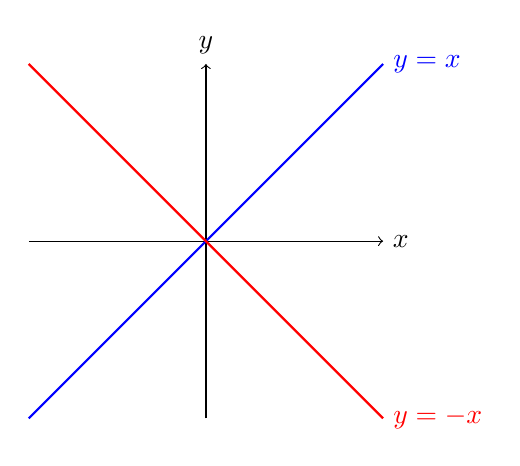
\begin{tikzpicture}[scale=0.75]
    % Axes
    \draw[->] (-3,0) -- (3,0) node[right] {\(x\)};
    \draw[->] (0,-3) -- (0,3) node[above] {\(y\)};

    % Droite y = x
    \draw[blue, thick] (-3,-3) -- (3,3) node[right] {\(y = x\)};

    % Droite y = -x
    \draw[red, thick] (-3,3) -- (3,-3) node[right] {\(y = -x\)};
    
\end{tikzpicture}
\end{center}
On voit que sur chaque point de la droite rouge, si on les ramènes sur la droite bleu (en faisant la projection) il arrive au point $(0, 0)$.
\end{exemple}







